\experiment{Page Replacement Algorithms}{11/10/2023}

\section{Aim}
Implement the page replacement algorithms a) FIFO b) LRU c) LFU

\section{Algorithm}
\subsection{First In First Out (FIFO)}
\begin{enumerate}
   \item Start
   \item Input the number of frames and the size of the reference string.
   \item Input the reference string and store it in the "s" array.
   \item Iterate over the reference string "s". For each page "pg" in the reference string:
   \begin{enumerate}
       \item If the page is not in the queue, increment the "fault" counter.
       \item If the queue is full, remove the page at the front of the queue.
       \item Enqueue the current page to the end of the queue.
   \end{enumerate}
   \item Print the number of page faults.
   \item Stop
\end{enumerate}

\subsection{Least Recently Used (LRU)}
\begin{enumerate}
   \item Start
   \item Input the number of frames and the size of the reference string.
   \item Input the reference string and store it in the "s" array.
   \item Iterate over the reference string "s". For each page "pg" in the reference string:
   \begin{enumerate}
       \item Search for the current page
       \item If the page is not in the memory:
       \begin{enumerate}
           \item Increment the "fault" counter.
           \item If the memory is full, remove the least recently used page.
           \item Add the current page to the memory.
       \end{enumerate}
       \item If the page is already in memory, place the current page at the top and remove it from the current position.
   \end{enumerate}
   \item Print the number of page faults.
   \item Stop
\end{enumerate}

\subsection{Least Frequently Used (LFU)}
\begin{enumerate}
   \item Start
   \item Input the number of frames and the size of the reference string.
   \item Input the reference string and store it in the "s" array.
   \item Iterate over the reference string "s". For each page "pg" in the reference string:
   \begin{enumerate}
       \item Search for the current page
       \item If the page is not in the memory:
       \begin{enumerate}
           \item Increment the "fault" counter.
           \item If the memory is full, remove the least frequently used page.
           \item Add the current page to the memory.
       \end{enumerate}
       \item If the page is already in memory, increment current page's count value
   \end{enumerate}
   \item Print the number of page faults.
   \item Stop
\end{enumerate}


\section{C Program - FIFO}
\begin{lstlisting}[label={list:c_program:queue}]
#include <stdio.h>

int s[20], n, q[100], f = -1, r = -1, fault = 0, pg = 0;

void enqueue(int item) {
    if (r == 99) {
        printf("Queue is full\n");
        return;
    }
    if (f == -1 && r == -1) {
        f = r = 0;
    } else {
        r++;
    }
    q[r] = item;
    fault++;
}

void dequeue() {
    if (f == -1 && r == -1) {
        printf("Queue is empty\n");
        return;
    }
    f++;
}

int search(int item) {
    int i;
    for (i = f; i <= r; i++) {
        if (q[i] == item) {
            return 1;
        }
    }
    return 0;
}

int main() {
    int no;

    printf("Input number of frames: ");
    scanf("%d", &n);

    printf("Input reference string size: ");
    scanf("%d", &no);

    printf("Input reference string: ");
    for (int i = 0; i < no; i++) {
        scanf("%d", &s[i]);
    }

    enqueue(s[0]);

    for (int i = 1; i < no; i++) {
        pg = s[i];
        if (search(pg) == 0) {
            if (r - f + 1 == n) {
                dequeue();
            }
            enqueue(pg);
        }
    }

    printf("Number of page faults: %d\n", fault);

    return 0;
}
\end{lstlisting}

\section{C Program - LRU}
\begin{lstlisting}[label={list:c_program:queue}]
#include <stdio.h>

int s[20], n, stack[100], top = -1, fault = 0;

void push(int item) {
    if (top == 99) {
        printf("Stack is full\n");
        return;
    }
    stack[++top] = item;
    fault++;
}

void pop_from_bottom() {
    if (top == -1) {
        printf("Stack is empty\n");
        return;
    }
    for (int i = 0; i < top; i++) {
        stack[i] = stack[i + 1];
    }
    top--;
}

int search(int item) {
    for (int i = 0; i <= top; i++) {
        if (stack[i] == item) {
            return i;
        }
    }
    return -1;
}

int main() {
    int no;

    printf("Input number of frames: ");
    scanf("%d", &n);

    printf("Input reference string size: ");
    scanf("%d", &no);

    printf("Input reference string: ");
    for (int i = 0; i < no; i++) {
        scanf("%d", &s[i]);
    }

    push(s[0]);

    for (int i = 1; i < no; i++) {
        int page_no = s[i];
        int index = search(page_no);

        if (index == -1) {
            if (top == n - 1) {
                pop_from_bottom();
            }
            push(page_no);
        } else {
            int temp = stack[index];
            for (int j = index; j < top; j++) {
                stack[j] = stack[j + 1];
            }
            stack[top] = temp;
        }
    }

    printf("Number of page faults: %d\n", fault);

    return 0;
}
\end{lstlisting}


\section{C Program - LFU}
\begin{lstlisting}[label={list:c_program:queue}]
#include <stdio.h>

int s[20], size = 0, fault = 0, n;

struct pages_in_memory {
    int page_no;
    int count;
} pages[20], page;

void remove_page() {
    int min_count = pages[0].count;
    int min_index = 0;

    for (int i = 1; i < size; i++) {
        if (pages[i].count < min_count) {
            min_count = pages[i].count;
            min_index = i;
        }
    }

    for (int i = min_index; i < size - 1; i++) {
        pages[i] = pages[i + 1];
    }

    size--;
}

void add_page(int item) {
    fault++;
    page.page_no = item;
    page.count = 1;

    if (size == n) {
        remove_page();
    }

    pages[size] = page;
    size++;
}

int search(int item) {
    for (int i = 0; i < size; i++) {
        if (pages[i].page_no == item) {
            return 1;
        }
    }
    return 0;
}

int main() {
    int no;

    printf("Input number of frames: ");
    scanf("%d", &n);

    printf("Input reference string size: ");
    scanf("%d", &no);

    printf("Input reference string: ");
    for (int i = 0; i < no; i++) {
        scanf("%d", &s[i]);
    }

    add_page(s[0]);

    for (int i = 1; i < no; i++) {
        int pno = s[i];
        if (search(pno) == 0) {
            add_page(pno);
        } else {
            for (int j = 0; j < size; j++) {
                if (pages[j].page_no == pno) {
                    pages[j].count++;
                    break;
                }
            }
        }
    }

    printf("\nNumber of page faults: %d\n", fault);

    return 0;
}
\end{lstlisting}


\section{Output}
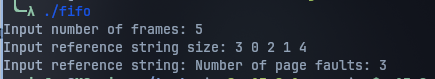
\includegraphics[width=0.5\linewidth]{Cycle_3//Outputs/fifo.png}
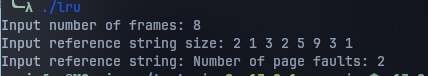
\includegraphics[width=0.5\linewidth]{Cycle_3//Outputs/lru.png}
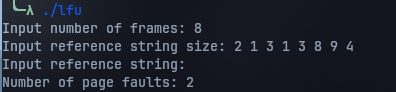
\includegraphics[width=0.5\linewidth]{Cycle_3//Outputs/lfu.png}

\section{Result}
Executed Page Replacement algorithms successfully